% Provenance (never printed): lycee terminale S SVT "Les climats de la Terre"
% and the 2019 enseignement scientifique ("Le climat de la Terre": forcing,
% feedbacks, the IPCC assessments, scenarios), union; physical science only,
% as the user ruled (2026-10-22). See sources/outline_sources.md. Pilot
% chapter, 2026-10-22. Every figure about the climate system is an IPCC AR6
% WG1 statement (ledger ipcc:*) or computed from a dataset in
% figdata/grade-12/climate_records.py.
\chapter{जलवायु परिवर्तन: प्रेक्षण, कारण और प्रक्षेपण}\label{ch:g12:climate-change}

प्रशांत महासागर के बीच के एक ज्वालामुखी, मौना लोआ, के उत्तरी ढाल पर ऊँचाई पर,
सफ़ेद इमारतों का एक समूह नंगे लावा पर खड़ा है,
समुद्र से \qty{3397}{m} ऊपर। वहाँ ऊपर, नीचे के द्वीप द्वारा प्रदूषित वायु की परत के
ऊपर और किसी भी बड़े शहर से हज़ारों किलोमीटर दूर, वायु
लगभग उतनी ही स्वच्छ और भली-भाँति मिश्रित है जितना पूरे ग्रह का वायुमंडल।
मार्च 1958 से उसकी कार्बन डाइऑक्साइड लगभग बिना रुकावट मापी जाती रही है।
अभिलेख एक रसायनज्ञ की परियोजना के रूप में शुरू हुआ; वह पृथ्वी-विज्ञान का सबसे प्रसिद्ध
वक्र बन गया है। यह अध्याय उस वक्र और जलवायु के दूसरे अभिलेखों को
पढ़ता है, समझाता है कि वायु में परिवर्तन ग्रह के \omterm{def:g10:earth-energy-budget:energy-budget}{ऊर्जा बजट} को कैसे
बदलता है, वैज्ञानिक कैसे तय करते हैं कि उनके द्वारा प्रेक्षित तापन का कारण क्या था,
और वे आने वाले दशकों के लिए क्या प्रक्षेपित करते हैं।
% ledger: noaa:mlo-site, noaa:keeling-1958

\begin{omfigure}
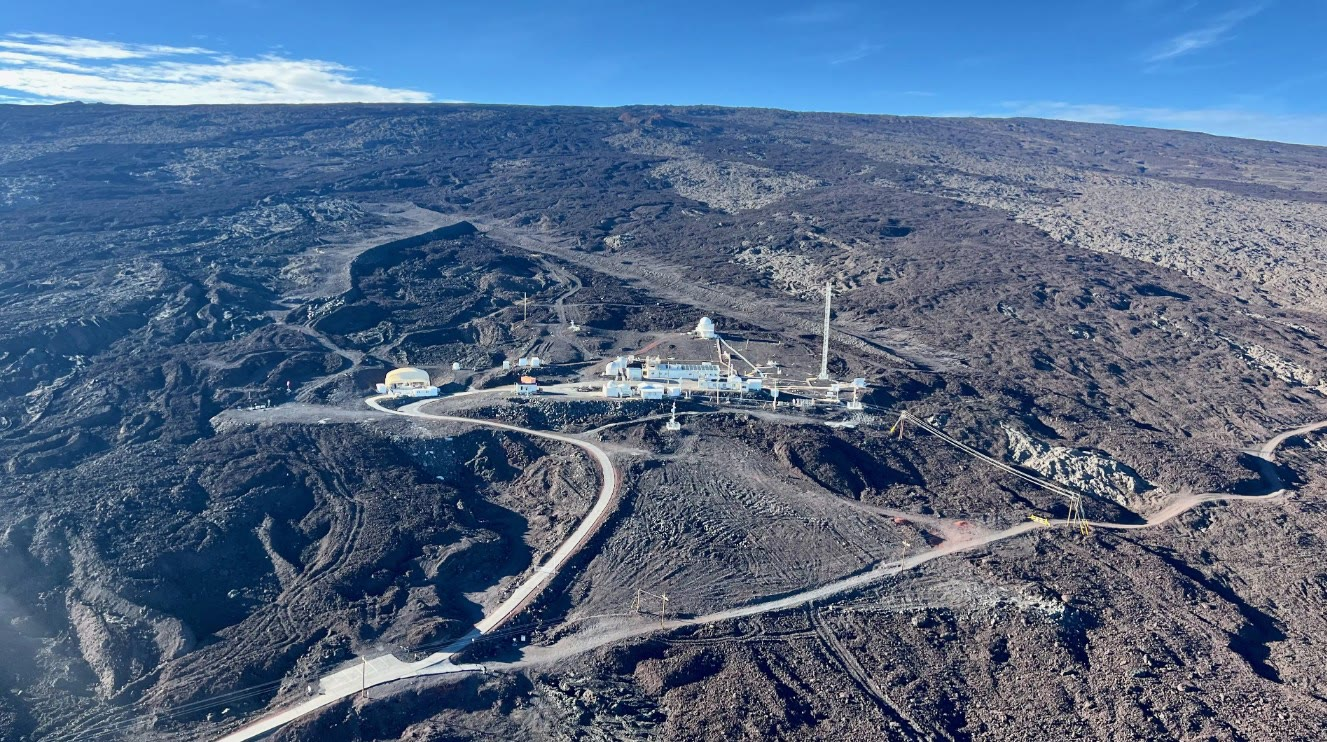
\includegraphics[width=0.78\linewidth]{images/book2/g12-noaa-mauna-loa-observatory.jpg}

{\small मौना लोआ वेधशाला, हवाई, ज्वालामुखी के उत्तरी पार्श्व पर ऊँचाई पर पुराने
लावा-प्रवाहों पर। फ़ोटो: ब्रायन वेज़ल, NOAA (सार्वजनिक डोमेन)।}
\end{omfigure}

\begin{recall}
पृथ्वी सूर्य से प्रकाश के रूप में ऊर्जा पाती है और औसतन उतनी ही मात्रा
अवरक्त विकिरण के रूप में अंतरिक्ष में खोती है; परावर्तित सूर्य-प्रकाश का अंश
\omterm{def:g10:earth-energy-budget:albedo}{एल्बिडो} है (\cref{ch:g10:earth-energy-budget})। ग्रीनहाउस गैसें --- जल-वाष्प,
कार्बन डाइऑक्साइड, मीथेन --- सतह द्वारा उत्सर्जित अवरक्त का एक भाग अवशोषित करती हैं
और उसका एक भाग वापस नीचे भेजती हैं; यह ग्रीनहाउस प्रभाव
सतह को उससे कहीं अधिक गरम रखता है जितनी वह अन्यथा होती (रसायन की पुस्तकें, और
पुस्तक 1, कक्षा 9)। \omterm{def:g12:past-climates:ice-core}{बर्फ़ के कोर} प्राचीन वायु के बुलबुले रखते हैं और पिछले 800\,000 वर्षों के
\omterm{def:g12:past-climates:glacial-cycle}{हिमनदीय चक्रों} को दर्ज करते हैं (\cref{ch:g12:past-climates})।
\end{recall}

\section{अभिलेख}

\begin{omfigure}
\begin{tikzpicture}
\begin{axis}[omrecord, width=0.92\linewidth, height=6.2cm, xmin=1957, xmax=2028,
  ymin=305, ymax=440, xlabel={वर्ष}, ylabel={कार्बन डाइऑक्साइड (ppm)},
  xtick={1960,1970,...,2020}, /pgf/number format/1000 sep={}]
\addplot[omDef!85!black, line width=0.5pt] table[x=decimal_year, y=co2_ppm] {figdata/out/grade-12-climate_records-co2.dat};
\addplot[only marks, mark=*, mark size=0.9pt, omThm!85!black] table[x=year, y=co2_ppm] {figdata/out/grade-12-climate_records-co2annual.dat};
\end{axis}
\end{tikzpicture}

{\small मौना लोआ पर वायु में कार्बन डाइऑक्साइड की मात्रा: मासिक माध्य
(रेखा) और वार्षिक माध्य (बिंदु), शुष्क वायु के प्रति दस लाख भागों (ppm) में।
आँकड़े: NOAA वैश्विक निगरानी प्रयोगशाला और स्क्रिप्स समुद्रविज्ञान
संस्थान।}
\end{omfigure}

\begin{proposition}[कार्बन डाइऑक्साइड का अभिलेख]\label{prop:g12:climate-change:co2}
% ledger: data:co2-mlo (all numbers computed in figdata/grade-12/climate_records.py)
मौना लोआ पर, कार्बन डाइऑक्साइड की वार्षिक माध्य सांद्रता 1959 के
\qty{316.0}{ppm} से 2025 में \qty{427.4}{ppm} तक बढ़ी, और वृद्धि
तेज़ होती जा रही है: 1960 के दशक में सांद्रता लगभग \qty{0.9}{ppm} प्रति वर्ष
और 2015 और 2025 के बीच लगभग \qty{2.6}{ppm} प्रति वर्ष बढ़ी। हर
वर्ष सांद्रता लगभग \qty{7}{ppm} ऊपर-नीचे भी होती है: वह मई में सबसे ऊँची
और सितंबर में सबसे नीची होती है।
\end{proposition}

\begin{remark}[वक्र के दाँते क्यों हैं]\label{rem:g12:climate-change:teeth}
वार्षिक उतार-चढ़ाव उत्तरी गोलार्ध की वनस्पति की साँस है,
जहाँ अधिकांश स्थलीय पौधे हैं। वसंत और गर्मियों में पौधे
प्रकाशसंश्लेषण द्वारा उससे अधिक कार्बन डाइऑक्साइड ग्रहण करते हैं जितनी वे और मृदा छोड़ते हैं;
पतझड़ और सर्दियों में अपघटन और श्वसन भारी पड़ते हैं। वर्ष-दर-वर्ष की
वृद्धि एक अलग कहानी है: वह जीवाश्म ईंधनों और साफ़ किए गए
वनों का कार्बन है जो वायु में जमा हो रहा है।
\end{remark}

\begin{proposition}[कम से कम दो मिलियन वर्षों में सबसे ऊँची]\label{prop:g12:climate-change:icecore}
% ledger: data:co2-bereiter (173.7 and 298.6 ppm computed), ipcc:co2-2myr (high confidence)
पिछले 800\,000 वर्षों में, अंटार्कटिक बर्फ़ के वायु-बुलबुले
कार्बन डाइऑक्साइड की सांद्रताएँ सबसे ठंडे \omterm{def:g12:past-climates:glacial-cycle}{हिमनदीय कालों} में लगभग \qty{174}{ppm}
और सबसे गरम \omterm{def:g12:past-climates:glacial-cycle}{अंतर्हिमनदीय कालों} में \qty{299}{ppm} के बीच दर्ज करते हैं। आज का
मान उनमें से सबसे ऊँचे से \qty{100}{ppm} से भी अधिक ऊपर है।
आकलन बताते हैं कि 2019 में सांद्रता कम से कम दो मिलियन वर्षों में किसी भी समय से
अधिक थी (\emph{उच्च विश्वास})।
\end{proposition}

\begin{omfigure}
\begin{tikzpicture}
\begin{axis}[omrecord, omage, width=0.92\linewidth, height=5.2cm, xmin=0, xmax=810,
  ymin=150, ymax=490, xlabel={1950 से पहले के हज़ार वर्ष},
  ylabel={कार्बन डाइऑक्साइड (ppm)}, xtick={0,100,...,800}]
\addplot[omDef!85!black, line width=0.6pt] table[x=age_kyr, y=co2_ppm] {figdata/out/grade-12-climate_records-icecore.dat};
\draw[omThm, densely dashed, line width=0.8pt] (axis cs:810,427.35) -- (axis cs:0,427.35);
\node[font=\footnotesize, text=omThm!85!black, anchor=south west] at (axis cs:780,433) {2025 में मौना लोआ पर वार्षिक माध्य};
\end{axis}
\end{tikzpicture}

{\small 800\,000 वर्षों में अंटार्कटिक बर्फ़ में कार्बन डाइऑक्साइड: \omterm{def:g12:past-climates:glacial-cycle}{हिमनदीय
चक्र} उसे लगभग 180 और \qty{300}{ppm} के बीच ले जाते हैं।
दाएँ सिरे पर पतली नुकीली रेखा सबसे नई बर्फ़ है, जो वर्तमान
वृद्धि की शुरुआत को, वर्ष 2001 तक, दर्ज करती है। आँकड़े: बेराइटर और अन्य (2015), NOAA
पुराजलवायु विज्ञान।}
% the youngest sample of the composite: age -51 yr BP (2001), 368.02 ppm (data/derived/co2-icecore.csv)
\end{omfigure}

\begin{omfigure}
\begin{tikzpicture}
\begin{axis}[omrecord, width=0.92\linewidth, height=5.6cm, xmin=1878, xmax=2027,
  ymin=-0.6, ymax=1.45, xlabel={वर्ष},
  ylabel={तापमान विसंगति (\unit{\degreeCelsius})},
  xtick={1880,1900,...,2020}, /pgf/number format/1000 sep={},
  legend style={at={(0.03,0.96)}, anchor=north west, font=\footnotesize, draw=black!30}]
\addplot[omDef!70, line width=0.5pt, mark=*, mark size=0.6pt] table[x=year, y=anomaly] {figdata/out/grade-12-climate_records-temp.dat};
\addlegendentry{वार्षिक माध्य}
\addplot[omThm!85!black, line width=1.3pt, unbounded coords=jump] table[x=year, y=mean11] {figdata/out/grade-12-climate_records-temp.dat};
\addlegendentry{11-वर्षीय औसत}
\end{axis}
\end{tikzpicture}

{\small वैश्विक माध्य सतह-तापमान, 1951--1980 के उसके औसत से अंतर के रूप में।
आँकड़े: नासा GISS सतह-तापमान विश्लेषण (GISTEMP v4)।}
\end{omfigure}

\begin{proposition}[प्रेक्षित वैश्विक तापन]\label{prop:g12:climate-change:warming}
% ledger: ipcc:gsat-2011-2020, ipcc:decades
पिछले चार दशकों में से हर एक 1850 के बाद के अपने से पहले के किसी भी दशक से अधिक
गरम रहा है। 2011--2020 का वैश्विक सतह-तापमान 1850--1900 के तापमान से \qty{1.09}{\degreeCelsius}
अधिक था (बहुत संभावित रूप से 0.95 और
\qty{1.20}{\degreeCelsius} के बीच), स्थल पर अधिक तापन के साथ
(\qty{1.59}{\degreeCelsius}) महासागर की तुलना में (\qty{0.88}{\degreeCelsius})।
\end{proposition}

\begin{proposition}[समुद्र-तल अधिकाधिक तेज़ी से उठता है]\label{prop:g12:climate-change:sea}
% ledger: ipcc:sea-level-obs, data:gmsl-lsa (3.2 mm/yr trend computed)
वैश्विक माध्य समुद्र-तल 1901 और 2018 के बीच लगभग \qty{0.20}{m} उठा।
दर 1901 से 1971 तक लगभग \qty{1.3}{mm} प्रति वर्ष,
1971 से 2006 तक \qty{1.9}{mm} प्रति वर्ष और 2006 से
2018 तक \qty{3.7}{mm} प्रति वर्ष थी (\emph{उच्च विश्वास})। 1993 से समुद्र-सतह की
ऊँचाई मापने वाले उपग्रह
1993--2025 में \qty{3.2}{mm} प्रति वर्ष का औसत पाते हैं। समुद्र इसलिए उठता है कि गरम होता
महासागर फैलता है और हिमनद और हिमचादरें उसमें बर्फ़ खोती हैं।
\end{proposition}

\begin{omfigure}
\begin{tikzpicture}
\begin{axis}[omrecord, width=0.86\linewidth, height=5cm, xmin=1992, xmax=2026,
  ymin=-35, ymax=95, xlabel={वर्ष}, ylabel={समुद्र-तल (mm)},
  /pgf/number format/1000 sep={}, xtick={1995,2000,...,2025}]
\addplot[omDef!85!black, line width=0.5pt] table[x=decimal_year, y=gmsl_mm] {figdata/out/grade-12-climate_records-sea.dat};
\end{axis}
\end{tikzpicture}

{\small अंतरिक्ष से लगभग हर दस दिन पर मापा गया वैश्विक माध्य समुद्र-तल
(मौसमी संकेत हटाकर), एक मनमाने शून्य के सापेक्ष। तुंगतामिति आँकड़े
NOAA उपग्रह तुंगतामिति प्रयोगशाला द्वारा उपलब्ध कराए गए हैं।}
\end{omfigure}

\begin{dated}{2025}
% ledger: data:co2-mlo, data:gistemp (values read from the datasets as fetched 2026-10-22)
2025 में मौना लोआ पर कार्बन डाइऑक्साइड की वार्षिक माध्य सांद्रता
\qty{427.35}{ppm} थी। नासा के तापमान-अभिलेख में अब तक का सबसे गरम वर्ष
2024 था, 1951--1980 के औसत से \qty{1.28}{\degreeCelsius} ऊपर।
\end{dated}

\section{विकिरणी प्रणोदन}

\begin{definition}[विकिरणी प्रणोदन]\label{def:g12:climate-change:forcing}
जलवायु तंत्र में किसी परिवर्तन --- अधिक ग्रीनहाउस गैस, अधिक एरोसॉल कण, अधिक चमकीला
सूर्य --- का \emph{विकिरणी प्रणोदन}\index{विकिरणी प्रणोदन} वह परिवर्तन है जो वह
वायुमंडल के शीर्ष पर जलवायु तंत्र में प्रवेश करने वाले ऊर्जा के शुद्ध प्रवाह में उत्पन्न करता है,
इससे पहले कि सतह के तापमान को प्रतिक्रिया का समय मिले। इसे पृथ्वी की सतह के प्रति वर्ग मीटर
वॉट (\unit{W/m^2}) में मापा जाता है। धनात्मक प्रणोदन से ग्रह
ऊर्जा प्राप्त करता है और गरम होता है; ऋणात्मक प्रणोदन से वह ऊर्जा खोता है और ठंडा होता है।
\end{definition}

\begin{remark}[प्रभावी प्रणोदन]\label{rem:g12:climate-change:effective}
आकलन \emph{प्रभावी} \omterm{def:g12:climate-change:forcing}{विकिरणी प्रणोदन} का उपयोग करते हैं, जो वायुमंडल
के तीव्र समायोजनों (उदाहरण के लिए उसके बादलों के) को भी गिनता है
जो सतह के गरम होने से पहले होते हैं। इस अध्याय के सभी \omterm{def:g12:climate-change:forcing}{प्रणोदन}
प्रभावी \omterm{def:g12:climate-change:forcing}{प्रणोदन} हैं।
\end{remark}

\begin{proposition}[1750 से प्रणोदन]\label{prop:g12:climate-change:forcing}
% ledger: ipcc:erf-total, ipcc:erf-agents
मानवीय गतिविधियों ने 1750 के सापेक्ष 2019 में
\qty{2.72}{W/m^2} का कुल \omterm{def:g12:climate-change:forcing}{विकिरणी प्रणोदन} उत्पन्न किया है (बहुत संभावित रूप से 1.96 और
\qty{3.48}{W/m^2} के बीच)। ग्रीनहाउस गैसें धनात्मक \omterm{def:g12:climate-change:forcing}{प्रणोदन} देती हैं, जिसमें सबसे आगे
कार्बन डाइऑक्साइड है (\qty{2.16}{W/m^2}); एरोसॉल कण, जो
सूर्य-प्रकाश परावर्तित करते हैं और बादलों को अधिक चमकीला बनाते हैं, ऋणात्मक \omterm{def:g12:climate-change:forcing}{प्रणोदन} देते हैं (कुल मिलाकर लगभग
\qty{-1.06}{W/m^2})। उसी अवधि में सूर्य की चमक में परिवर्तन
केवल \qty{0.01}{W/m^2} देता है।
\end{proposition}

\begin{omfigure}
% ledger: ipcc:erf-agents, ipcc:erf-total (central values and 5-95 % ranges of AR6 Table 7.8)
\begin{tikzpicture}
\begin{axis}[xbar, width=0.8\linewidth, height=7.2cm, xmin=-1.8, xmax=3.7,
  ytick={1,...,10}, yticklabels={कुल (मानवीय), सौर, भूमि-उपयोग,
  एरोसॉल--बादल, एरोसॉल--विकिरण, ओज़ोन, हैलोजनित गैसें, नाइट्रस ऑक्साइड,
  मीथेन, कार्बन डाइऑक्साइड}, y tick label style={font=\small},
  tick label style={font=\small}, xlabel={प्रभावी विकिरणी प्रणोदन, 1750--2019 (\unit{W/m^2})},
  label style={font=\small}, bar width=6pt, bar shift=0pt, axis x line=bottom, axis y line=left,
  axis line style={-}, enlarge y limits=0.07, xmajorgrids,
  grid style={gray!22, line width=0.3pt}, extra x ticks={0},
  extra x tick style={grid style={black!60, line width=0.5pt}}]
\addplot[fill=omThm!55, draw=omThm!80!black, error bars/.cd, x dir=both, x explicit,
  error bar style={black!70}] coordinates {
  (2.16,10) += (0.25,0) -= (0.26,0)
  (0.54,9) += (0.11,0) -= (0.11,0)
  (0.21,8) += (0.03,0) -= (0.03,0)
  (0.41,7) += (0.08,0) -= (0.08,0)
  (0.47,6) += (0.24,0) -= (0.23,0)
  (2.72,1) += (0.76,0) -= (0.76,0)
  (0.01,2) += (0.07,0) -= (0.07,0)};
\addplot[fill=omDef!55, draw=omDef!80!black, error bars/.cd, x dir=both, x explicit,
  error bar style={black!70}] coordinates {
  (-0.22,5) += (0.26,0) -= (0.25,0)
  (-0.84,4) += (0.59,0) -= (0.61,0)
  (-0.20,3) += (0.10,0) -= (0.10,0)};
\end{axis}
\end{tikzpicture}

{\small 1750 से 2019 तक के मुख्य प्रभावी \omterm{def:g12:climate-change:forcing}{विकिरणी प्रणोदन}, अपने
बहुत संभावित परासों (मूँछें) के साथ। मान: IPCC छठी आकलन रिपोर्ट, कार्य
समूह~I, तालिका 7.8।}
\end{omfigure}

\begin{proposition}[कार्बन डाइऑक्साइड: हर दोगुनापन वही प्रणोदन जोड़ता है]\label{prop:g12:climate-change:log}
% ledger: ipcc:erf-2xco2, ipcc:log-co2
अच्छे सन्निकटन तक, कार्बन डाइऑक्साइड का \omterm{def:g12:climate-change:forcing}{प्रणोदन} उसकी सांद्रता के
\emph{लघुगणक} के साथ बढ़ता है: हर दोगुनापन वही \omterm{def:g12:climate-change:forcing}{प्रणोदन} जोड़ता है,
$F_{2\times} = \qty{3.93}{W/m^2}$, जब सांद्रता 1750 के मान, $C_0 = \qty{278}{ppm}$, से दोगुनी हो।
किसी सांद्रता $C$ का \omterm{def:g12:climate-change:forcing}{प्रणोदन} तब है
\[
  F = F_{2\times}\,\frac{\ln (C/C_0)}{\ln 2}.
\]
\end{proposition}

\begin{example}[आकलन के सापेक्ष नियम की जाँच]\label{ex:g12:climate-change:check}
% ledger: ipcc:erf-2xco2, ipcc:erf-agents
2019 में सांद्रता \qty{410}{ppm} थी। नियम देता है
$F = 3.93 \times \ln(410/278)/\ln 2 = 3.93 \times 0.561 \approx
\qty{2.20}{W/m^2}$, जो उस \qty{2.16}{W/m^2} के 2\,\% के भीतर है जो
आकलन 1750--2019 के लिए कार्बन डाइऑक्साइड को देता है।
\end{example}

\begin{proposition}[अतिरिक्त ऊर्जा कहाँ जाती है]\label{prop:g12:climate-change:heating}
% ledger: ipcc:heating
चूँकि \omterm{def:g12:climate-change:forcing}{प्रणोदन} धनात्मक है, जलवायु तंत्र ऊर्जा प्राप्त करता है: 2006--2018 में
औसतन लगभग \qty{0.79}{W/m^2}, जो 1971--2006 के \qty{0.50}{W/m^2} से
अधिक है (\emph{उच्च विश्वास})। इस ऊर्जा का 91\,\% महासागर ने लिया;
स्थल ने 5\,\%, पिघलती बर्फ़ ने 3\,\% और वायुमंडल ने केवल 1\,\%।
\end{proposition}

\section{प्रतिपुष्टियाँ और जलवायु संवेदनशीलता}

जब सतह गरम होती है, तो वह अंतरिक्ष में अधिक ऊर्जा विकिरित करती है, जो ग्रह को
वापस संतुलन में लाने की प्रवृत्ति रखती है। पर तापन दूसरी चीज़ें भी
बदलता है --- वायु में जल-वाष्प, भूमि पर हिम और बर्फ़,
बादल --- और ये परिवर्तन अपनी बारी में \omterm{def:g10:earth-energy-budget:energy-budget}{ऊर्जा बजट} को बदलते हैं।

\begin{definition}[जलवायु प्रतिपुष्टि]\label{def:g12:climate-change:feedback}
\emph{जलवायु प्रतिपुष्टि}\index{जलवायु प्रतिपुष्टि} जलवायु तंत्र में तापमान-परिवर्तन
से उत्पन्न कोई ऐसा परिवर्तन है जो \omterm{def:g10:earth-energy-budget:energy-budget}{ऊर्जा बजट} को, और इसलिए स्वयं
तापमान-परिवर्तन को, बदल देता है। \emph{धनात्मक प्रतिपुष्टि} प्रारंभिक
परिवर्तन को बढ़ाती है; \emph{ऋणात्मक प्रतिपुष्टि} उसे मंद करती है।
\end{definition}

\begin{example}[तीन प्रतिपुष्टियाँ]\label{ex:g12:climate-change:three}
\begin{itemize}
  \item \textbf{जल-वाष्प (धनात्मक)।} गरम वायु अधिक जल-वाष्प
        रखती है, जो एक ग्रीनहाउस गैस है, और इससे तापन बढ़ता है।
  \item \textbf{हिम और बर्फ़ (धनात्मक)।} हिम और बर्फ़ सूर्य-प्रकाश परावर्तित करते हैं;
        जब वे पिघलते हैं, तो नीचे की गहरी रंग की भूमि और समुद्र उसका अधिक भाग अवशोषित करते हैं,
        और तापन बढ़ता है।
  \item \textbf{अंतरिक्ष में विकिरण (ऋणात्मक)।} अधिक गरम सतह और
        वायुमंडल अंतरिक्ष में अधिक अवरक्त विकिरित करते हैं। यह मूल प्रतिक्रिया
        अंत में हमेशा जीतती है: इसीलिए जलवायु बिना सीमा के गरम होने के बजाय
        एक नए, अधिक गरम संतुलन पर टिक जाती है।
\end{itemize}
\end{example}

\begin{omfigure}
\begin{tikzpicture}[font=\small, >={Stealth[length=2.4mm]},
  box/.style={draw=black!60, rounded corners=2pt, fill=white, align=center,
  inner sep=3pt, text width=3cm}]
  \node[box, fill=omThm!12] (w) at (0,0) {सतह गरम होती है};
  \node[box] (v) at (3.6,1.3) {वायु में अधिक जल-वाष्प};
  \node[box] (g) at (3.6,-1.3) {अधिक प्रबल\\ग्रीनहाउस प्रभाव};
  \draw[->, omThm!85!black, thick] (w) to[bend left=18] (v);
  \draw[->, omThm!85!black, thick] (v) -- (g);
  \draw[->, omThm!85!black, thick] (g) to[bend left=18] (w);
  \node[font=\footnotesize, text=omThm!85!black] at (2.0,0) {$+$};
  \node[box] (s) at (-3.6,1.3) {हिम और बर्फ़ पिघलते हैं};
  \node[box] (a) at (-3.6,-1.3) {कम एल्बिडो: अधिक सूर्य-प्रकाश अवशोषित};
  \draw[->, omThm!85!black, thick] (w) to[bend right=18] (s);
  \draw[->, omThm!85!black, thick] (s) -- (a);
  \draw[->, omThm!85!black, thick] (a) to[bend right=18] (w);
  \node[font=\footnotesize, text=omThm!85!black] at (-2.0,0) {$+$};
  \node[box] (r) at (0,-2.9) {अंतरिक्ष में अधिक अवरक्त विकिरित};
  \draw[->, omDef!85!black, thick] ([xshift=-0.35cm]w.south) -- ([xshift=-0.35cm]r.north);
  \draw[->, omDef!85!black, thick] ([xshift=0.35cm]r.north) -- ([xshift=0.35cm]w.south);
  \node[font=\footnotesize, text=omDef!85!black] at (0.62,-1.45) {$-$};
\end{tikzpicture}

{\small दो धनात्मक \omterm{def:g12:climate-change:feedback}{प्रतिपुष्टियाँ} (लाल लूप) तापन को बढ़ाती हैं; अधिक गरम ग्रह
द्वारा विकिरित अतिरिक्त अवरक्त (नीला) एक ऋणात्मक \omterm{def:g12:climate-change:feedback}{प्रतिपुष्टि} है जो
उसे सीमित करती है।}
\end{omfigure}

\begin{proposition}[साम्य पर तापन]\label{prop:g12:climate-change:equilibrium}
% ledger: ipcc:feedbacks
जब जलवायु एक नए संतुलन पर पहुँच जाती है, तो किसी स्थिर \omterm{def:g12:climate-change:forcing}{प्रणोदन} से उत्पन्न तापन $\Delta T$,
जहाँ \omterm{def:g12:climate-change:forcing}{प्रणोदन} $F$ है, यह होता है
\[
  \Delta T = \frac{F}{\lambda},
\]
जहाँ $\lambda$, \emph{\omterm{def:g12:climate-change:feedback}{जलवायु प्रतिपुष्टि} प्राचल}, वह अतिरिक्त ऊर्जा है
जो ग्रह तापन की हर डिग्री के लिए अंतरिक्ष में खोता है। आकलन
अंतरिक्ष में विकिरण ($\qty{3.22}{W.m^{-2}.\degreeCelsius^{-1}}$)
को जल-वाष्प और तापमान-प्रोफ़ाइल की धनात्मक \omterm{def:g12:climate-change:feedback}{प्रतिपुष्टियों}
($1.30$), सतह \omterm{def:g10:earth-energy-budget:albedo}{एल्बिडो} की ($0.35$) और बादलों की ($0.42$, उसी
इकाई में) के साथ मिलाकर $\lambda \approx \qty{1.16}{W.m^{-2}.\degreeCelsius^{-1}}$ पाते हैं।
\end{proposition}

\begin{proof}[आंशिक उपपत्ति]
नए संतुलन पर जलवायु तंत्र फिर से अंतरिक्ष में उतनी ही ऊर्जा खोता है
जितनी वह प्राप्त करता है, इसलिए तापन के कारण होने वाली अतिरिक्त हानि, $\lambda\,\Delta T$, को
\omterm{def:g12:climate-change:forcing}{प्रणोदन} की भरपाई करनी चाहिए: $\lambda\,\Delta T = F$। यह कि अतिरिक्त हानि
$\Delta T$ के समानुपाती है, एक सन्निकटन है, जो कुछ डिग्री के तापन के लिए अच्छा है,
और यहाँ मान लिया गया है।
\end{proof}

\begin{definition}[साम्य जलवायु संवेदनशीलता]\label{def:g12:climate-change:ecs}
\emph{साम्य जलवायु संवेदनशीलता}\index{साम्य जलवायु संवेदनशीलता}
कार्बन डाइऑक्साइड की सांद्रता को उसके 1750 के स्तर से दोगुना करने के बाद,
नया संतुलन प्राप्त होने पर, पृथ्वी की सतह का तापन है।
\end{definition}

\begin{proposition}[जलवायु कितनी संवेदनशील है?]\label{prop:g12:climate-change:ecs}
% ledger: ipcc:ecs
प्रमाण की सभी पंक्तियों --- \omterm{def:g12:climate-change:feedback}{प्रतिपुष्टियों} की भौतिकी,
प्रेक्षित तापन, अतीत की जलवायु --- को मिलाकर, आकलन \omterm{def:g12:climate-change:ecs}{साम्य जलवायु संवेदनशीलता} का
सर्वोत्तम अनुमान \qty{3}{\degreeCelsius} देते हैं, संभावित रूप से
2.5 और \qty{4}{\degreeCelsius} के बीच (\emph{उच्च विश्वास}), और बहुत
संभावित रूप से 2 और \qty{5}{\degreeCelsius} के बीच।
\end{proposition}

\section{ज़िम्मेदार कौन है?}

\begin{method}[आकलनों का कोई कथन पढ़ना]\label{met:g12:climate-change:language}
% ledger: ipcc:likelihood
जलवायु विज्ञान के अंतरराष्ट्रीय आकलन हर निष्कर्ष को एक निश्चित शब्दावली में श्रेणीबद्ध करते हैं,
जो तिरछे अक्षरों में छपती है:
\begin{itemize}
  \item \emph{संभाव्यता}, किसी परिणाम की प्रायिकता:
        \emph{लगभग निश्चित} 99--100\,\%, \emph{अत्यंत संभावित}
        95--100\,\%, \emph{बहुत संभावित} 90--100\,\%, \emph{संभावित}
        66--100\,\%, \emph{जितना संभावित उतना ही असंभावित} 33--66\,\%,
        \emph{असंभावित} 0--33\,\%, \emph{बहुत असंभावित} 0--10\,\%;
  \item \emph{विश्वास}, किसी निष्कर्ष के पीछे के प्रमाण की प्रबलता और
        सहमति: बहुत निम्न, निम्न, मध्यम, उच्च, बहुत उच्च।
\end{itemize}
$[x \text{ से } y]$ लिखा गया परास एक बहुत संभावित परास है: 90\,\%
संभावना है कि सही मान उसके भीतर है। किसी कथन को पढ़ने के लिए
राशि, उसका सर्वोत्तम अनुमान, उसका परास, और उससे जुड़ी संभाव्यता या
विश्वास पहचानिए।
\end{method}

\begin{definition}[आरोपण]\label{def:g12:climate-change:attribution}
\emph{आरोपण}\index{आरोपण} यह आकलन है कि किसी
प्रेक्षित परिवर्तन का कितना भाग उसके हर संभावित कारण के कारण है, परिणाम की
संभाव्यता के साथ।
\end{definition}

\begin{proposition}[मानवीय प्रभाव]\label{prop:g12:climate-change:attribution}
% ledger: ipcc:unequivocal, ipcc:attribution, ipcc:observed-2010-2019
यह असंदिग्ध है कि मानवीय प्रभाव ने वायुमंडल, महासागर
और स्थल को गरम किया है। 1850--1900 और 2010--2019 के बीच, वैश्विक सतह
लगभग \qty{1.06}{\degreeCelsius} गरम हुई। मानवीय गतिविधियों ने
\qty{0.8}{\degreeCelsius} से \qty{1.3}{\degreeCelsius} का तापन किया (संभावित परास), सर्वोत्तम
अनुमान \qty{1.07}{\degreeCelsius}: भली-भाँति मिश्रित ग्रीनहाउस गैसों ने संभावित रूप से
सतह को 1.0 से \qty{2.0}{\degreeCelsius} गरम किया, और दूसरे मानवीय
प्रभावों ने, मुख्यतः एरोसॉल ने, संभावित रूप से उसे 0 से
\qty{0.8}{\degreeCelsius} ठंडा किया। सूर्य और ज्वालामुखियों ने उसे केवल $-0.1$
से $+\qty{0.1}{\degreeCelsius}$ बदला, और जलवायु के प्राकृतिक उतार-चढ़ाव ने
$-0.2$ से $+\qty{0.2}{\degreeCelsius}$।
\end{proposition}

\begin{omfigure}
% ledger: ipcc:attribution, ipcc:observed-2010-2019
\begin{tikzpicture}
\begin{axis}[width=0.7\linewidth, height=5.6cm, xmin=-1, xmax=2.2, ymin=0.4, ymax=6.6,
  ytick={1,...,6}, yticklabels={प्राकृतिक परिवर्तनशीलता, सूर्य और ज्वालामुखी,
  एरोसॉल और अन्य मानवीय, ग्रीनहाउस गैसें, सभी मानवीय प्रभाव, प्रेक्षित},
  y tick label style={font=\small}, tick label style={font=\small},
  xlabel={1850--1900 से 2010--2019 तक के तापन में योगदान (\unit{\degreeCelsius})},
  label style={font=\small}, axis x line=bottom, axis y line=left, axis line style={-},
  xmajorgrids, grid style={gray!22, line width=0.3pt}, extra x ticks={0},
  extra x tick style={grid style={black!60, line width=0.5pt}}]
\draw[black!70, line width=5pt] (axis cs:0.88,6) -- (axis cs:1.21,6);
\fill (axis cs:1.06,6) circle (2.4pt);
\draw[omThm!80, line width=5pt] (axis cs:0.8,5) -- (axis cs:1.3,5);
\fill (axis cs:1.07,5) circle (2.4pt);
\draw[omThm!55, line width=5pt] (axis cs:1.0,4) -- (axis cs:2.0,4);
\draw[omDef!60, line width=5pt] (axis cs:-0.8,3) -- (axis cs:0,3);
\draw[gray!70, line width=5pt] (axis cs:-0.1,2) -- (axis cs:0.1,2);
\draw[gray!45, line width=5pt] (axis cs:-0.2,1) -- (axis cs:0.2,1);
\end{axis}
\end{tikzpicture}

{\small प्रेक्षित तापन का कारण क्या था: हर योगदान के संभावित परास,
जहाँ आकलन सर्वोत्तम अनुमान देता है वहाँ उसके साथ (बिंदु); प्रेक्षित
तापन के लिए उसका बहुत संभावित परास। मान: IPCC छठी आकलन
रिपोर्ट, कार्य समूह~I, नीति-निर्माताओं के लिए सारांश, A.1.3।}
\end{omfigure}

\section{परिदृश्य और प्रक्षेपण}

\begin{definition}[परिदृश्य और प्रक्षेपण]\label{def:g12:climate-change:scenario}
\emph{उत्सर्जन परिदृश्य}\index{उत्सर्जन परिदृश्य} इसकी एक सुसंगत
कहानी है कि ग्रीनहाउस गैसों और एरोसॉल के उत्सर्जन भविष्य में कैसे
बदल सकते हैं। \emph{प्रक्षेपण}\index{प्रक्षेपण (जलवायु)} किसी दिए गए परिदृश्य के लिए
मॉडलों द्वारा परिकलित जलवायु की प्रतिक्रिया है। प्रक्षेपण
पूर्वानुमान नहीं है: वह बताता है कि क्या होता \emph{यदि} परिदृश्य सच हो जाए।
\end{definition}

\begin{proposition}[प्रक्षेपित तापन और समुद्र-तल वृद्धि]\label{prop:g12:climate-change:projections}
% ledger: ipcc:proj-temp, ipcc:proj-sea, ipcc:3myr
आकलन पाँच मुख्य \omterm{def:g12:climate-change:scenario}{परिदृश्यों} का उपयोग करते हैं, बहुत कम उत्सर्जनों (SSP1-1.9)
से बहुत अधिक उत्सर्जनों (SSP5-8.5) तक। 2081--2100 के लिए, 1850--1900 की तुलना में,
वे नीचे दिए तापन प्रक्षेपित करते हैं (सर्वोत्तम अनुमान और बहुत संभावित परास,
\unit{\degreeCelsius} में), और, 2100 तक, 1995--2014 के सापेक्ष वैश्विक माध्य समुद्र-तल की
संभावित वृद्धियाँ। हर \omterm{def:g12:climate-change:scenario}{परिदृश्य} में समुद्र पूरी शताब्दी उठता
रहता है (\emph{लगभग निश्चित})। पिछली बार वैश्विक
सतह 1850--1900 से \qty{2.5}{\degreeCelsius} या अधिक ऊपर तीन मिलियन वर्ष से भी
पहले रही थी (\emph{मध्यम विश्वास})।

\begin{center}
\small
\begin{tabular}{lccc}
\hline
\omterm{def:g12:climate-change:scenario}{परिदृश्य} & उत्सर्जन & तापन 2081--2100 (\unit{\degreeCelsius}) & 2100 तक समुद्र-तल वृद्धि (m) \\
\hline
SSP1-1.9 & बहुत कम & 1.4 (1.0 से 1.8) & 0.28 से 0.55 \\
SSP1-2.6 & कम & 1.8 (1.3 से 2.4) & 0.32 से 0.62 \\
SSP2-4.5 & मध्यवर्ती & 2.7 (2.1 से 3.5) & 0.44 से 0.76 \\
SSP3-7.0 & अधिक & 3.6 (2.8 से 4.6) & --- \\
SSP5-8.5 & बहुत अधिक & 4.4 (3.3 से 5.7) & 0.63 से 1.01 \\
\hline
\end{tabular}
\end{center}
\end{proposition}

\begin{omfigure}
% ledger: ipcc:proj-temp
\begin{tikzpicture}
\begin{axis}[width=0.8\linewidth, height=5.2cm, xmin=0.4, xmax=5.6, ymin=0, ymax=6.2,
  xtick={1,...,5}, xticklabels={SSP1-1.9, SSP1-2.6, SSP2-4.5, SSP3-7.0, SSP5-8.5},
  x tick label style={font=\small}, tick label style={font=\small},
  ylabel={तापन 2081--2100 (\unit{\degreeCelsius})}, label style={font=\small},
  axis x line=bottom, axis y line=left, axis line style={-}, ymajorgrids,
  grid style={gray!22, line width=0.3pt}]
\draw[omThm!60, line width=9pt] (axis cs:1,1.0) -- (axis cs:1,1.8);
\draw[black, line width=1.2pt] (axis cs:0.83,1.4) -- (axis cs:1.17,1.4);
\draw[omThm!60, line width=9pt] (axis cs:2,1.3) -- (axis cs:2,2.4);
\draw[black, line width=1.2pt] (axis cs:1.83,1.8) -- (axis cs:2.17,1.8);
\draw[omThm!60, line width=9pt] (axis cs:3,2.1) -- (axis cs:3,3.5);
\draw[black, line width=1.2pt] (axis cs:2.83,2.7) -- (axis cs:3.17,2.7);
\draw[omThm!60, line width=9pt] (axis cs:4,2.8) -- (axis cs:4,4.6);
\draw[black, line width=1.2pt] (axis cs:3.83,3.6) -- (axis cs:4.17,3.6);
\draw[omThm!60, line width=9pt] (axis cs:5,3.3) -- (axis cs:5,5.7);
\draw[black, line width=1.2pt] (axis cs:4.83,4.4) -- (axis cs:5.17,4.4);
\end{axis}
\end{tikzpicture}

{\small पाँचों \omterm{def:g12:climate-change:scenario}{परिदृश्यों} के लिए शताब्दी के अंत में प्रक्षेपित तापन:
बहुत संभावित परास (पट्टी) और सर्वोत्तम अनुमान (काली रेखा)। मान: IPCC छठी
आकलन रिपोर्ट, कार्य समूह~I, तालिका SPM.1।}
\end{omfigure}

\begin{remark}[यह अध्याय क्या नहीं कहता]\label{rem:g12:climate-change:science}
विश्व कौन-सा \omterm{def:g12:climate-change:scenario}{परिदृश्य} अपनाएगा, यह भविष्य के उत्सर्जनों पर, यानी
ऐसे निर्णयों पर निर्भर है जो भौतिकी के प्रश्न नहीं हैं। भौतिक विज्ञान बताता है
कि जलवायु हर एक पर कैसी प्रतिक्रिया करती है; उनके बीच चुनाव
समाजों का है, और उसकी लागतों और लाभों का अध्ययन दूसरे विज्ञान करते हैं।
\end{remark}

\begin{history}[एक वक्र जो एक रसायनज्ञ की परियोजना के रूप में शुरू हुआ]
% ledger: noaa:keeling-1958
मार्च 1958 में स्क्रिप्स समुद्रविज्ञान संस्थान के रसायनज्ञ चार्ल्स डेविड कीलिंग ने
मौना लोआ पर वायु की कार्बन डाइऑक्साइड को
ऐसे उपकरण से मापना शुरू किया जो प्रति दस लाख भागों में एक भाग के अंश जितने परिवर्तन देख सके।
कुछ ही वर्षों में उनके अभिलेख ने वनस्पति की वार्षिक साँस
और एक स्थिर वृद्धि, दोनों दिखाईं। तब से
स्क्रिप्स और अमेरिका की मौसम और महासागर एजेंसी द्वारा जारी मापन वायुमंडल की संरचना का
सबसे लंबा प्रत्यक्ष अभिलेख हैं।
\begin{center}
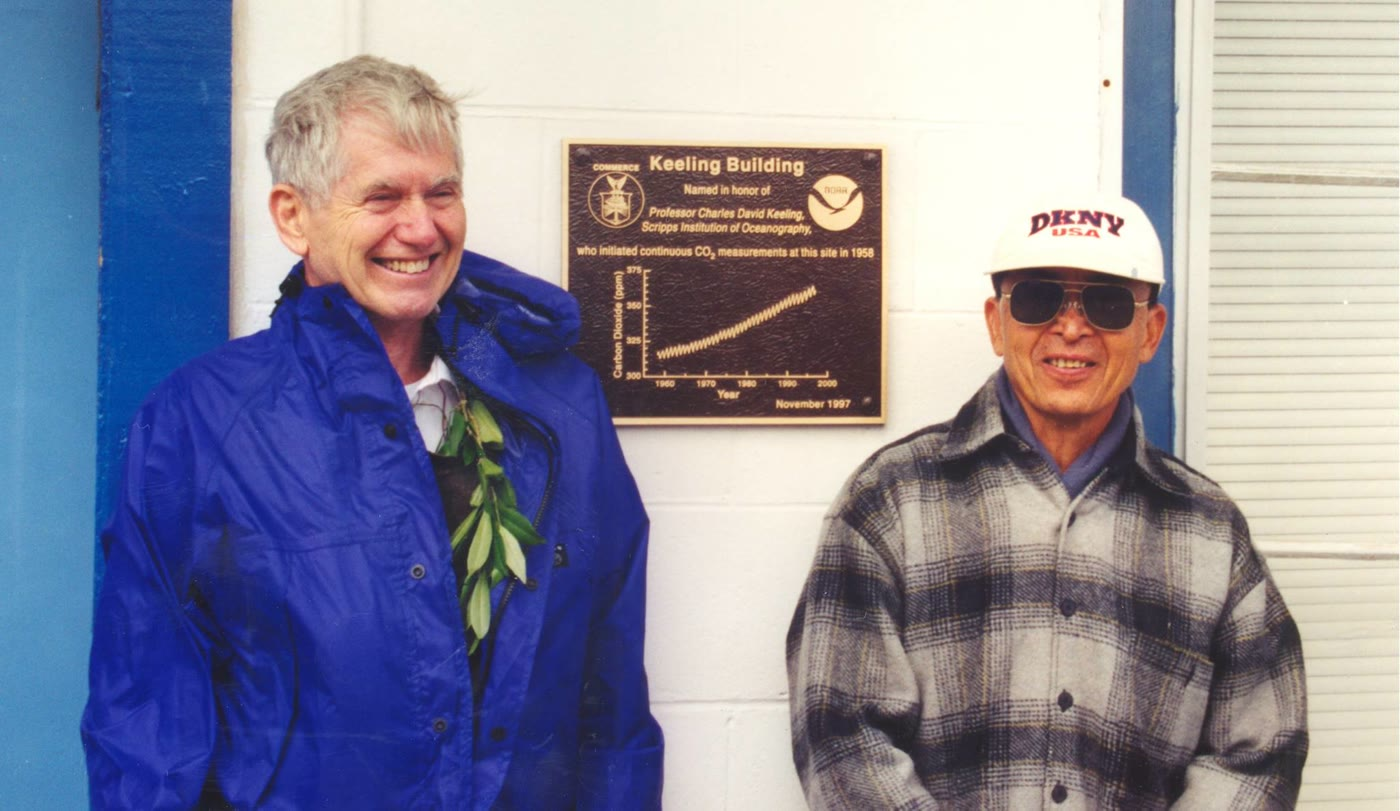
\includegraphics[width=0.62\linewidth]{images/book2/g12-noaa-keeling-chin-1997.jpg}

{\small चार्ल्स डेविड कीलिंग (बाएँ) और जॉन चिन 1997 में मौना लोआ
वेधशाला पर, उस पट्टिका के पास जो एक इमारत का नाम कीलिंग के नाम पर रखती है।
फ़ोटो: जॉन मिलर, NOAA (सार्वजनिक डोमेन)।}
\end{center}
\end{history}

\section{अभ्यास}

\begin{exercise}[$\star$]\label{exo:g12:climate-change:1}
जलवायु तंत्र में किसी परिवर्तन का \omterm{def:g12:climate-change:forcing}{विकिरणी प्रणोदन} क्या है? उसे किस
इकाई में मापा जाता है, और उसके चिह्न का क्या अर्थ है?
\end{exercise}

\begin{exercise}[$\star$]\label{exo:g12:climate-change:2}
वर्ष के किस महीने में मौना लोआ पर कार्बन डाइऑक्साइड की सांद्रता
सबसे ऊँची होती है, और किसमें सबसे नीची? वार्षिक उतार-चढ़ाव समझाइए।
\end{exercise}

\begin{exercise}[$\star$]\label{exo:g12:climate-change:3}
आकलनों की शब्दावली में, \emph{बहुत
संभावित} का अर्थ कौन-सी प्रायिकता है? और \emph{संभावित} का? $[0.95 \text{ से } 1.20]$
लिखे गए परास का क्या अर्थ है?
\end{exercise}

\begin{exercise}[$\star$]\label{exo:g12:climate-change:4}
हाल के दशकों में जलवायु तंत्र द्वारा प्राप्त अतिरिक्त ऊर्जा का
कितना अंश महासागर में गया? इससे यह क्यों समझ आता है कि समुद्र-तल
बर्फ़ पिघले बिना भी उठता है?
\end{exercise}

\begin{exercise}[$\star$]\label{exo:g12:climate-change:5}
दो धनात्मक \omterm{def:g12:climate-change:feedback}{जलवायु प्रतिपुष्टियाँ} और वह ऋणात्मक प्रतिक्रिया बताइए जो
तापन को सीमित करती है। हर एक को एक वाक्य में समझाइए।
\end{exercise}

\begin{exercise}[$\star\star$]\label{exo:g12:climate-change:6}
मौना लोआ पर कार्बन डाइऑक्साइड की वार्षिक माध्य सांद्रता 1959 में
\qty{315.98}{ppm} और 2025 में \qty{427.35}{ppm} थी। वह कितने ppm,
और कितने प्रतिशत बढ़ी? पूरी अवधि में प्रति वर्ष औसत वृद्धि
कितनी थी?
\end{exercise}

\begin{exercise}[$\star\star$]\label{exo:g12:climate-change:7}
अध्याय के लघुगणकीय नियम का उपयोग करके, $F_{2\times} =
\qty{3.93}{W/m^2}$ और $C_0 = \qty{278}{ppm}$ लेकर, 2025 के वार्षिक माध्य
\qty{427.35}{ppm} पर कार्बन डाइऑक्साइड का \omterm{def:g12:climate-change:forcing}{प्रणोदन} परिकलित कीजिए।
\end{exercise}

\begin{exercise}[$\star\star$]\label{exo:g12:climate-change:8}
\qty{3.7}{mm} प्रति वर्ष पर, जो 2006--2018 की दर है, 30 वर्षों में समुद्र-तल कितना
उठेगा? यह दर 1901--1971 की दर, \qty{1.3}{mm} प्रति वर्ष, से कितने गुना
तेज़ है?
\end{exercise}

\begin{exercise}[$\star\star$]\label{exo:g12:climate-change:9}
$\Delta T = F/\lambda$ का उपयोग करके, जहाँ $\lambda = \qty{1.16}{W.m^{-2}.\degreeCelsius^{-1}}$,
वह साम्य तापन परिकलित कीजिए जो 2019 का कुल मानवीय \omterm{def:g12:climate-change:forcing}{प्रणोदन},
\qty{2.72}{W/m^2}, उत्पन्न करता। प्रेक्षित मानव-जनित तापन केवल
लगभग \qty{1.07}{\degreeCelsius} है। अंतर का मुख्य कारण बताइए।
\end{exercise}

\begin{exercise}[$\star\star$]\label{exo:g12:climate-change:10}
सूर्य और ज्वालामुखियों ने 1850--1900 और 2010--2019 के बीच वैश्विक तापमान को
$-0.1$ से $+\qty{0.1}{\degreeCelsius}$ बदला, जबकि प्रेक्षित
तापन लगभग \qty{1.06}{\degreeCelsius} था। आप क्या निष्कर्ष निकाल सकते हैं? किस
दूसरे प्राकृतिक कारण को भी नकारना होगा, और आकलन उसके बारे में
क्या कहता है?
\end{exercise}

\begin{exercise}[$\star\star$]\label{exo:g12:climate-change:11}
\omterm{def:g12:climate-change:scenario}{प्रक्षेपणों} की तालिका का उपयोग करके, किन \omterm{def:g12:climate-change:scenario}{परिदृश्यों} में 2081--2100 का तापन
बहुत संभावित रूप से \qty{2}{\degreeCelsius} से नीचे रहता है? किसमें वह
बहुत संभावित रूप से \qty{2}{\degreeCelsius} से अधिक होता है?
\end{exercise}

\begin{exercise}[$\star\star\star$]\label{exo:g12:climate-change:12}
एरोसॉल ने लगभग $-0.22$ और $\qty{-0.84}{W/m^2}$ का \omterm{def:g12:climate-change:forcing}{प्रणोदन} उत्पन्न किया
(सूर्य-प्रकाश के माध्यम से और बादलों के माध्यम से)। यदि सभी एरोसॉल वायु से हटा दिए
जाएँ जबकि बाक़ी सब 2019 जैसा रहे, तो कुल मानवीय
\omterm{def:g12:climate-change:forcing}{प्रणोदन} क्या हो जाएगा? $\lambda = \qty{1.16}{W.m^{-2}.\degreeCelsius^{-1}}$ के साथ,
साम्य तापन कितना बढ़ेगा?
\end{exercise}

\begin{exercise}[$\star\star\star$]\label{exo:g12:climate-change:13}
लघुगणकीय नियम से दिखाइए कि \qty{278}{ppm} से
\qty{556}{ppm} तक जाना और \qty{556}{ppm} से \qty{1112}{ppm} तक जाना वही
\omterm{def:g12:climate-change:forcing}{प्रणोदन} जोड़ते हैं। \qty{1112}{ppm} पर कुल \omterm{def:g12:climate-change:forcing}{प्रणोदन} क्या है?
\end{exercise}

\begin{exercise}[$\star\star\star$]\label{exo:g12:climate-change:14}
लघुगणकीय नियम का $C$ के सापेक्ष अवकलन कीजिए। \qty{280}{ppm} पर कार्बन डाइऑक्साइड का
एक अतिरिक्त ppm कितना \omterm{def:g12:climate-change:forcing}{प्रणोदन} जोड़ता है, और
\qty{420}{ppm} पर कितना? टिप्पणी कीजिए।
\end{exercise}

\begin{exercise}[$\star\star\star$]\label{exo:g12:climate-change:15}
अंतरिक्ष में अतिरिक्त विकिरण के सिवाय किसी \omterm{def:g12:climate-change:feedback}{प्रतिपुष्टि} के बिना,
$\lambda_0 = \qty{3.22}{W.m^{-2}.\degreeCelsius^{-1}}$। कार्बन डाइऑक्साइड के दोगुना होने
($F_{2\times} = \qty{3.93}{W/m^2}$) के लिए तापन
$\lambda_0$ के साथ, फिर $\lambda = \qty{1.16}{W.m^{-2}.\degreeCelsius^{-1}}$ के साथ परिकलित कीजिए।
\omterm{def:g12:climate-change:feedback}{प्रतिपुष्टियाँ} तापन को कितने गुणक से बढ़ाती हैं?
\end{exercise}

\section{समस्या: संख्याओं में कीलिंग वक्र}

\begin{problem}[{सप्ताहांत समस्या --- वनस्पति की वार्षिक साँस से
उस वर्ष तक जब दोगुनापन पहुँचेगा}]
\label{pb:g12:climate-change:1}
% ledger: data:co2-mlo (annual means 1960 316.91, 1970 325.68, 2015 401.01,
% 2025 427.35; seasonal departures May +3.37, September -3.51, means of
% 2015-2024; all from figdata/grade-12/climate_records.py), noaa:mlo-site,
% ipcc:erf-2xco2, ipcc:ecs, ipcc:feedbacks, ipcc:co2-2myr
एक विद्यार्थी मौना लोआ का अभिलेख डाउनलोड करता है और एक
स्प्रेडशीट के साथ उस पर काम करता है। 2015--2024 में, मासिक सांद्रता मई में औसतन
समतलित प्रवृत्ति से \qty{3.37}{ppm} ऊपर और सितंबर में उससे \qty{3.51}{ppm} नीचे
रहती है। वार्षिक माध्य 1960 में \qty{316.91}{ppm},
1970 में \qty{325.68}{ppm}, 2015 में \qty{401.01}{ppm} और 2025 में \qty{427.35}{ppm}
हैं। 1750 की सांद्रता \qty{278}{ppm} थी। $F_{2\times} = \qty{3.93}{W/m^2}$
के साथ लघुगणकीय नियम का उपयोग कीजिए।

\medskip
\noindent\textbf{भाग I --- वनस्पति की साँस।}
\begin{enumerate}
  \item वार्षिक चक्र का शिखर से गर्त तक का आयाम क्या है?
  \item समझाइए कि सांद्रता मई में सबसे ऊँची और सितंबर में
        सबसे नीची क्यों होती है।
  \item दक्षिणी गोलार्ध की वायु में चक्र कहीं अधिक कमज़ोर है।
        इसका कारण सुझाइए।
  \item वेधशाला \qty{3397}{m} की ऊँचाई पर, प्रशांत के बीच
        एक ज्वालामुखी पर, क्यों बनाई गई?
\end{enumerate}

\medskip
\noindent\textbf{भाग II --- प्रवृत्ति।}
\begin{enumerate}[resume]
  \item 1960--1970 में औसत वृद्धि, ppm प्रति वर्ष में, परिकलित कीजिए।
  \item इसे 2015--2025 के लिए परिकलित कीजिए।
  \item वृद्धि-दर कितने गुणक से बढ़ी है?
  \item 1750 और 2025 के बीच सांद्रता कितने प्रतिशत
        बढ़ी?
  \item \omterm{def:g12:past-climates:ice-core}{बर्फ़ के कोर} पिछले 800\,000 वर्षों में कभी लगभग \qty{300}{ppm} से अधिक
        नहीं दिखाते। 2025 का मान इससे कितने ppm
        अधिक है?
\end{enumerate}

\medskip
\noindent\textbf{भाग III --- प्रणोदन।}
\begin{enumerate}[resume]
  \item 2025 में कार्बन डाइऑक्साइड का \omterm{def:g12:climate-change:forcing}{प्रणोदन} परिकलित कीजिए।
  \item इसे 1960 के लिए परिकलित कीजिए, और 1960
        और 2025 के बीच \omterm{def:g12:climate-change:forcing}{प्रणोदन} की वृद्धि भी।
  \item कौन-सी सांद्रता 2025 के \omterm{def:g12:climate-change:forcing}{प्रणोदन} में \qty{1}{W/m^2} जोड़ेगी?
  \item 2015--2025 की वृद्धि-दर पर, इसमें कितने वर्ष लगेंगे?
\end{enumerate}

\medskip
\noindent\textbf{भाग IV --- दोगुनापन।}
\begin{enumerate}[resume]
  \item 1750 के मान के दोगुने की सांद्रता क्या है? वह कौन-सा
        \omterm{def:g12:climate-change:forcing}{प्रणोदन} उत्पन्न करती है?
  \item \omterm{def:g12:climate-change:ecs}{साम्य जलवायु संवेदनशीलता} के सर्वोत्तम अनुमान के साथ,
        वह कौन-सा साम्य तापन उत्पन्न करेगी? संभावित परास दीजिए।
  \item \qty{3}{\degreeCelsius} की संवेदनशीलता कौन-सा \omterm{def:g12:climate-change:feedback}{प्रतिपुष्टि} प्राचल $\lambda$
        दर्शाती है? इसकी तुलना \omterm{def:g12:climate-change:feedback}{प्रतिपुष्टियों} को जोड़कर प्राप्त मान
        \qty{1.16}{W.m^{-2}.\degreeCelsius^{-1}} से
        कीजिए।
  \item जिस दिन दोगुनापन पहुँचेगा, उस दिन सतह इस तापन तक क्यों नहीं
        पहुँचेगी?
  \item आज की वृद्धि-दर को केवल आगे बढ़ाने वाला परिकलन एक
        \omterm{def:g12:climate-change:scenario}{परिदृश्य} क्यों है, और आकलनों द्वारा किए जाने वाले प्रकार का \omterm{def:g12:climate-change:scenario}{प्रक्षेपण} क्यों नहीं?
  \item यदि 2015--2025 की वृद्धि-दर वैसी ही रहे, तो 1750 की सांद्रता का
        दोगुनापन किस वर्ष पहुँचेगा?
\end{enumerate}
\end{problem}
